\documentclass[]{article}
\usepackage{amsmath, amsfonts}
\usepackage{enumitem}
\usepackage{fancyhdr}
\usepackage{geometry}
\usepackage{cancel}
\usepackage{graphicx}
\usepackage{color}
\usepackage{multirow}
\usepackage{float}
\usepackage{pgfplots}	% To draw charts directly in Latex
\usepackage{marvosym}	% For lightning symbol to denote contradiction
\usepackage{cleveref}	% For clever referencing :)
\usepackage{nameref}	% For referencing to the section name, not number

%TikZ package for drawing:
\usepackage{tikz}
%For calculation of coordinates:
\usetikzlibrary{calc}
\usetikzlibrary{positioning}

%opening
\title{Problem Set V \\ \large Microeconomics II}
\author{Nurfatima Jandarova}
\date{\today}
\pagestyle{fancy}

\lhead{Microeconomics II, Problem Set V}
\rhead{Nurfatima Jandarova}
\renewcommand{\headrulewidth}{0.4pt}
\fancyheadoffset{1 cm}

\geometry{a4paper, left=20mm, top=20mm, bottom = 20mm, headheight=20mm}

\sloppy
\definecolor{lightgray}{gray}{0.5}
\setlength{\parindent}{0pt}

\renewcommand{\arraystretch}{1.3}

\begin{document}

\maketitle

\subsection*{Exercise 1}
\subsubsection*{1.1}
\begin{figure}[h]
	\begin{center}
		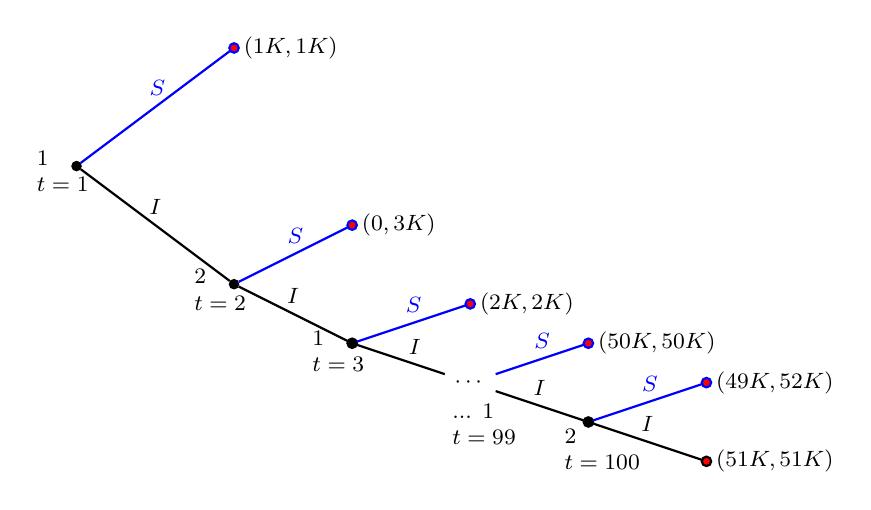
\begin{tikzpicture}
		[
		grow =right,
		font=\footnotesize,
		edge from parent/.style={draw,thick}
		]
		
		% Two node styles: solid and hollow
		\tikzstyle{solid node}=[circle,draw,inner sep=1.2,fill=black];
		\tikzstyle{end node}=[circle,draw,inner sep=1.2,fill=red];
		\tikzstyle{hollow node}=[circle,draw,inner sep=1.2];
		
		% Specify spacing for each level of the tree
		\tikzstyle{level 1}=[level distance=20mm,sibling distance=30mm]
		\tikzstyle{level 2}=[level distance=15mm,sibling distance=15mm]
		\tikzstyle{level 3}=[level distance=15mm,sibling distance=10mm]
		% The Tree
		\node(0)[solid node]{}
		% t=1, Invest
		child{node[solid node]{}
			% t = 2, Invest
			child{node[solid node]{}
				child {node {$\cdots$}
					child{node[solid node]{} 
						child{node[end node] {} edge from parent node [above]{$I$}}
						child{[blue] node[end node] {} edge from parent node [above]{$S$}}	
					edge from parent node[above]{$I$}}
					child{[blue] node[end node]{} edge from parent node[above]{$S$}}
				edge from parent node[align=left, xshift = 5, yshift = -2, above]{$I$}
				}
			% t = 3, Stop
				child{[blue] node[end node]{} edge from parent node[above]{$S$}}
				 edge from parent node[align=left, above]{$I$}
			}
			% t = 2, Stop
			child{[blue] node[end node]{} edge from parent node[align=left, above]{$S$}
			}
			edge from parent node[align=left, above]{$I$}
		}	
		% t=1, Stop
		child{[blue] node[end node]{} edge from parent node[align=left, above]{$S$}
		}
		;
		% Information sets
		% \draw[dotted,very thick](0-1-1)to(0-1-2);
		
		% Players
		% player 1, turn 1
		\node[align=left,yshift=-2, xshift=-5]at(0){1\\$t = 1$};
		% player 2, turn 2
		\node[align=left,yshift=-2, xshift=-5]at(0-1){2\\$t = 2$};
		% player 1, turn 3
		\node[align=left,yshift=-3, xshift=-5]at(0-1-1){1\\$t = 3$};
		\node[align=left,yshift=-15, xshift = 5]at(0-1-1-1){... 1\\$t=99$};
		\node[align=left,yshift=-10, xshift = 5]at(0-1-1-1-1){2\\$t=100$};
		
		% Specifying payoffs
		% Stop
		\node[right]at(0-2){$(1K, 1K)$};
		\node[right]at(0-1-2){$(0, 3K)$};
		\node[right]at(0-1-1-2){$(2K,2K)$};
		\node[right]at(0-1-1-1-2){$(50K,50K)$};
		\node[right]at(0-1-1-1-1-2){$(49K,52K)$};
		\node[right]at(0-1-1-1-1-1){$(51K,51K)$};
		\end{tikzpicture}
	\end{center}
	\caption{A centipede game in extensive form}
	\label{fig:ex1ext}
\end{figure}

There are two players, $N = \{1, 2\}$. According to the description of the game, all information sets in this game are singletons ($\#(H_1) = \#(H_2) = 50$). Therefore, strategy of a player has 50 elements (actions at all information sets of the player). Define the strategy spaces and payoff functions:
\begin{equation}
	\begin{split}
		S_1 = S_2 = \{I, S\}^{50} \\ \nonumber
		\pi_1: S_1\times S_2 \to 1000\{0, 1, ..., 51\} \\
		\pi_2: S_2\times S_1 \to 1000\{1, 2, ..., 52\} \\
	\end{split}
\end{equation}
Hence, the game in strategic form is given by
\begin{equation}
	G(\Gamma) = \{N, S_1\times S_2, \{\pi_1, \pi_2\}\} \nonumber
\end{equation}
and could be represented with a payoff matrix, excerpt of which is presented below
\begin{table}[h]
	\centering
	\begin{tabular}{c|ccccc}
		& I, I, ..., I & I, I, ..., S & ... & I, S, ..., S & S, S, ..., S \\
		\hline
		I, I, ..., I & (\underline{51K}, 51K)   & (49K, \underline{52K})   & ... & (1K, 4K)     & (0, 3K)      \\
		I, I, ..., S & (50K, 50K)   & (\underline{50K}, 50K)   & ... & (1K, 4K)     & (0, 3K)      \\
		$\vdots$       & \multicolumn{5}{c}{$\ddots$}                                      \\
		I, S, ..., S & (2K, 2K)     & (2K, 2K)     & ... & (\underline{2K}, 2K)     & (0, \underline{3K})      \\
		S, S, ..., S & (1K, \underline{1K})     & (1K, \underline{1K})     & ... & (1K, \underline{1K})     & (\underline{1K}, \underline{1K})
	\end{tabular}
	\caption{Part of payoff matrix of the game in strategic form}
	\label{tab:ex1str}
\end{table}

\subsubsection*{1.2}
I'm not sure how to search for Nash equilibria in mixed strategies here, so I present my reasoning for Nash equilibrium in pure strategies. As seen from the above table, if player 1 believes player 2 always invests, then it is optimal for the first player to always invest as well. However, if player 2 believes player 1 always invests it is optimal for him/her to stop at $t = 100$. So it cannot be a Nash equilibrium. Similarly, if player 1 believes 2 is going to play $(I, I, ..., I, S)$, his/her best response is to play $(I, I, ..., I, S)$, but given such belief about first player, the best response of the second player would be to stop at $t=98$, just one period before the other player stops. Continuing the same reasoning, it is clear that best responses of the two players intersect only when both of them choose $(S, S, ..., S, S)$. Hence, $\{(S, S, ..., S, S), (S, S, ..., S, S)\}$ is a Nash equilibrium in pure strategies.

By definition, a strategy is a subgame perfect equilibrium if it is NE in every perfect subgame of the game. Consider the smallest subgame at time $t=100$, where player 2 has to decide which action to take. The most optimal action for player 2 in this subgame is to stop and get \$52,000 instead of \$51,000 in case he/she chooses to invest. As mentioned earlier, both players prefer to stop just one period before they believe the other player wants to play stop. Then, in the subgame at $t=99$, it is optimal for player 1 to stop. Iterating backwards, we arrive at time $t = 1$, where again player 1 wants to stop because he/she knows that next period player 2 will play stop. Thus, $\{(S, S, ..., S, S), (S, S, ..., S, S)\}$ is also SGPE. This is also illustrated by blue lines in \Cref{fig:ex1ext}.

\subsection*{Exercise 2}

The strategic form representation of the game.
There are two players, i.e., $N = \{1, 2\}$. Their strategy spaces:
\begin{equation}
	\begin{split}
		S_1 = \{A, B, C\} \\ \nonumber
		S_2 = \{a, b\}
	\end{split}
\end{equation}
Profit matrix:
\begin{table}[h]
	\centering
	\begin{tabular}{c|cc}
		& a       & b       \\ \hline
		\makebox[0pt][l]{\rule[0.15cm]{0.2\textwidth}{0.7pt}}
		A & (-1, 1) & (1, 0)  \\
		B & (4, 0)  & (-4, 1) \\
		C & (2, 0)  & (2, 0) 
	\end{tabular}
\end{table}

Notice that strategy $A$ of player 1 is strictly dominated by a mixed strategy $\sigma_1 = (0, \frac{1}{7}, \frac{6}{7})$:
\begin{equation}
	\begin{split}
		\pi_1(\sigma_1, a) = -1\cdot0 + 4\frac{1}{7} + 2\frac{6}{7} > -1 = \pi_1(A, a) \\ \nonumber
		\pi_1(\sigma_1, b) = 1\cdot0 - 4\frac{1}{7} + 2\frac{6}{7} = \frac{8}{7} > 1 = \pi_1(A, b)
	\end{split}
\end{equation}

\subsubsection*{2.1}
\textit{Sorry, I forgot the question was only asking about NE in pure strategies and also found NE in mixed strategies. However, further on I only consider the NE in pure strategies that I've found.}

Using the fact that all Nash equilibria survive IESDS, we can restrict the search of NE to the remaining game. Define the mixed strategy of player 1, $\sigma_1 = (p, 1 - p)$, where $p$ is the probability of player 1 choosing action $B$; and the mixed strategy of player 2, $\sigma_2 = (q, 1 - q)$, where $q$ is the probability of player 2 playing a.

\begin{equation}
	\begin{split}
	\pi_1(\sigma_1, \sigma_2)& = q(4p + 2(1 - p)) + (1 - q)(-4p + 2(1 - p)) = 2 + 2p(4q - 3) \\ \nonumber
	\pi_2(\sigma_1, \sigma_2)& = p(1 - q) = p - pq \\
	\rho_1(\sigma_2)& = \begin{cases}
	0 & \text{ if }q < \frac{3}{4}\\
	[0, 1] & \text{ if }q = \frac{3}{4} \\
	1 & \text{ if }q > \frac{3}{4}\end{cases} \\
	\rho_2(\sigma_1)& = \begin{cases}
	0 & \text{ if }p > 0 \\
	[0, 1] & \text{ if }p = 0
	\end{cases}
	\end{split}
\end{equation}

The best response correspondences are depicted below in \Cref{fig:ex2br}.

\begin{figure}[h]
	\centering
	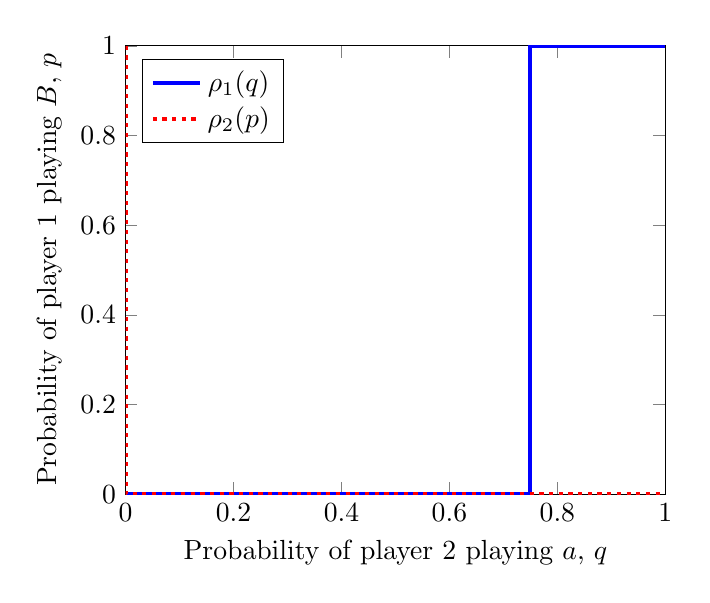
\begin{tikzpicture}
	\begin{axis}[
	xlabel={Probability of player 2 playing $a$, $q$},
	ylabel={Probability of player 1 playing $B$, $p$},
	xmin=0, xmax=1,
	ymin=0, ymax=1,
	legend pos=north west,
	ymajorgrids=false,
	]
	
	% Best response correspondence of player 1
	\addplot [color = blue, line width = 1.5pt]
	coordinates {(0,0)(3/4,0)(3/4,1)(1,1)};
	
	% Best response correspondence of player 2
	\addplot[color=red, line width = 1.5pt, dotted]
	coordinates {(0,1)(0,0)(1,0)};
	
	% Nash equilibria
%	\addplot[only marks, color=green, mark = *]
%	coordinates {(0,1)(2/3,1/3)(1,0)};
	\legend{$\rho_1(q)$, $\rho_2(p)$}
	\end{axis}
	\end{tikzpicture}
	\caption{Best response correspondences}
	\label{fig:ex2br}
\end{figure}

Hence, there is one Nash equilibrium in pure strategies, $(C, b)$ and a continuum of Nash equilibria in mixed strategies, $\sigma_1\times\sigma_2 = \{(0, 0, 1), (q, 1 - q)\}$, such that $q \leq \frac{3}{4}$.

\subsubsection*{2.2}
There is only one proper subgame: the entire game itself. Therefore, the NE $(C, b)$ is also a SGPE.

\subsubsection*{2.3}

Let $\mu$ denote the probability that player 2 assigns to being at the node following player 1 choosing $B$. Consequently, the belief of the second player that he/she is in the node induced by $A$ is $1 - \mu$.

Let's first find conditions for $\mu$ such that player 2 chooses $a$ over $b$ and vice versa:
\begin{equation*}
	\begin{aligned}[c]
		\text{Player 2 chooses }&a\text{ over $b$ if }\\
		\pi_2(a; \mu) = 1 - \mu& > \mu = \pi_2(b; \mu) \\
		\mu < \frac{1}{2}
	\end{aligned}
	\qquad\qquad\begin{aligned}
		\text{Player 2 chooses }&b\text{ over $a$ if }\\
		\pi_2(a; \mu) = 1 - \mu& < \mu = \pi_2(b; \mu) \\
		\mu > \frac{1}{2}
	\end{aligned}
\end{equation*}
Consider the first case, where $\mu < \frac{1}{2}$. Then, by sequential rationality, player 1 chooses $B$. This implies that given the strategy profile $(B, a)$, the ex-ante probability of reaching the information set of player 2 is 1 and ex-ante probability of reaching the node induced by $B$ is also equal to one. Then, $\mu < \frac{1}{2} < \frac{1}{1}$, which means that such system of beliefs is inconsistent. Hence, $(B, a)$ cannot be a WPBE.

Consider the second case, where $\mu > \frac{1}{2}$, i.e., player 2 chooses $b$ over $a$. Then, sequential rationality implies that the first player chooses $C$, in which case, the information set of the second player is never reached. Therefore, any system of beliefs of player 2 is statistically consistent. Hence, the strategy profile $(C, b)$ is a WPBE in pure strategies.

%%%%% Erased this as the question only asks about pure strategy WPBE.%%%%
%And finally, consider the case when $\mu = \frac{1}{2}$, i.e., player 2 is indifferent between $a$ and $b$. Denote the probability of player 2 choosing $a$ by $t$. Then, we must have that 
%\begin{equation}
%	\begin{split}
%		\pi_1(A; t) = -t + (1 - t)& = 4t - 4(1 - t) = \pi_1(B; t) \\ \nonumber
%		1 - 2t& = 8t - 4 \\
%		t = \frac{1}{2} \Longrightarrow \\
%		\pi_1(A; t) = \pi_1(B; t) = 0 < 2 = \pi_1(C)
%	\end{split}
%\end{equation}
%Once again, this implies that the probability of reaching the information set of player 2 is zero, hence

\subsection*{Exercise 3}
\subsubsection*{3.1}

First player has two information sets and his/her strategy space is $S_1 = \{A, B\}\times\{C, D\}$. Player 2 has one information set and his/her strategy space is $S_2 = \{a, b\}$.

\subsubsection*{3.2}
\begin{enumerate}[label=(\roman*)]
	\item To find NE in pure strategies, consider the matrix payoff with best responses in pure strategies underlined in \Cref{tab:ex3str}.
	\begin{table}[h]
		\begin{minipage}[b]{0.4\linewidth}
			\begin{tabular}{c|cc}
				& a 		& b 		\\ \hline
				A, C 	& (\underline{2}, \underline{-1}) 	& (-1, -2) 	\\
				A, D	& (-10, -2)	& (0, \underline{-1})	\\
				B, C 	& (1, \underline{1}) 	& (\underline{1}, \underline{1}) 	\\
				B, D	& (1, \underline{1})	& (\underline{1}, \underline{1})\\
			\end{tabular}
			\caption{Entire game in strategic form}
			\label{tab:ex3str}
		\end{minipage}\hfill
		\begin{minipage}[b]{0.4\linewidth}
			\begin{tabular}{c|cc}
				& a & b \\ \hline
				C & (\underline{2}, \underline{-1}) &  (-1, -2) \\
				D & (-10, -2) & (\underline{0}, \underline{-1})
			\end{tabular}
			\caption{NEs in second proper subgame}
			\label{tab:ex3psg2}
		\end{minipage}
	\end{table}
	
	Therefore, there are three NE in pure strategies: $\{(A, C, a), (B, C, b), (B, D, b)\}$.
	
	\item There are two proper subgames: entire game and subgame that starts at the node where player 2 has to choose an action. Consider the second proper subgame tabulated in \Cref{tab:ex3psg2}.	There are two NE in the second proper subgame, $\{(C, a), (D, b)\}$. The first player's best response to $(C, a)$ is to play $A$. Similarly, BR of the first player to $(D, b)$ is to choose $B$. Hence, there are two SGPE, $\{(A, C, a), (B, D, b)\}$.
	
	\item 	Let $\mu$ denote the probability player 1 assigns to being at the node induced by action $a$ of player 2. Then, 
	\begin{equation}
		\begin{split}
			\pi_1(C; \mu)& = 2\mu - (1 - \mu) = 3\mu - 1 \\ \nonumber
			\pi_1(D; \mu)& = -10\mu
		\end{split}
	\end{equation}
	Consider the case when $\mu > \frac{1}{13}$, i.e., player 1 chooses $C$ over $D$ in his/her second information set. Given this belief, sequential rationality implies that player 2 chooses $a$ and player 1 plays $A$ in the first information set. That is, given any belief system such that $\mu > \frac{1}{13}$, strategy $(A, C, a)$ is sequentially rational. This strategy, in turn, implies that the probability of reaching the second information set of player 1 is equal to 1 and probability of reaching the node induced by $a$ is also equal to 1. Then, the statistically consistent belief system would be $\mu = \frac{1}{1} = 1 > \frac{1}{13}$. Hence, a strategy $(A, C, a)$ and a belief system $(1, 0)$ constitute a WPBE.
	
	Consider another case, when $\mu < \frac{1}{13}$, i.e, when player 1 chooses $D$ over $C$. In this case, player 2 wants to play $b$ and player 1 prefers $B$ in the beginning of the game. Given, the strategy $(B, D, b)$, the second information set of player 1 is never reached. Hence, any belief system is consistent. Therefore, the strategy $(B, D, b)$ and any belief system such that $\mu < \frac{1}{13}$ constitute another WPBE.
	
	Thus, WPBE = SGPE.
\end{enumerate}

\subsubsection*{3.3}
\label{ex3.3}

The following game in extensive form (with imperfect recall) has the same strategic form representation as in \Cref{tab:ex3str}.

\begin{figure}[h]
	\begin{center}
		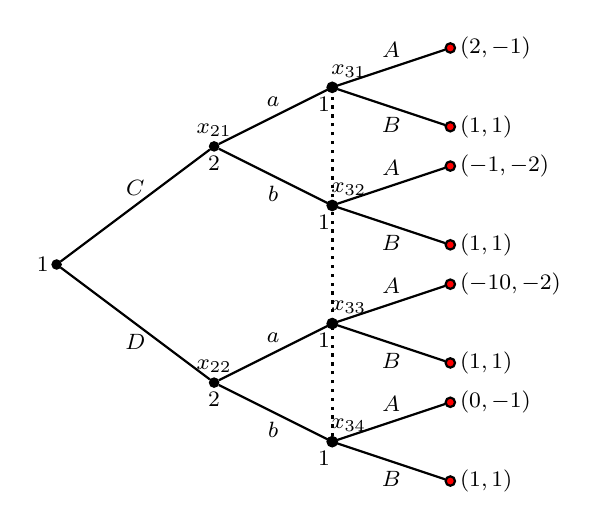
\begin{tikzpicture}
		[grow =right,
		font=\footnotesize,
		edge from parent/.style={draw,thick}
		]
		
		% Two node styles: solid and hollow
		\tikzstyle{solid node}=[circle,draw,inner sep=1.2,fill=black];
		\tikzstyle{end node}=[circle,draw,inner sep=1.2,fill=red];
		\tikzstyle{hollow node}=[circle,draw,inner sep=1.2];
		
		% Specify spacing for each level of the tree
		\tikzstyle{level 1}=[level distance=20mm,sibling distance=30mm]
		\tikzstyle{level 2}=[level distance=15mm,sibling distance=15mm]
		\tikzstyle{level 3}=[level distance=15mm,sibling distance=10mm]
		% The Tree
		\node(0)[solid node]{}
		% Player 1 D
		child{node[solid node]{}
			% Player 2
			child{node[solid node]{}
				% Player 1, A or B
				child{node[end node] {} edge from parent node[below]{$B$}}
				child{node[end node] {} edge from parent node[above]{$A$}}
				edge from parent node[below]{$b$}
			}
			child{node[solid node]{} 
				% Player 1, A or B
				child{node[end node] {} edge from parent node[below]{$B$}}
				child{node[end node] {} edge from parent node[above]{$A$}}
				edge from parent node[above]{$a$}
			}
			edge from parent node[below]{$D$}
		}
		% Player 1 C
		child{node[solid node]{}
			% Player 2
			child{node[solid node]{}
				% Player 1, A or B
				child{node[end node] {} edge from parent node[below]{$B$}}
				child{node[end node] {} edge from parent node[above]{$A$}}
				edge from parent node[below]{$b$}
			}
			child{node[solid node]{} 
				% Player 1, A or B
				child{node[end node] {} edge from parent node[below]{$B$}}
				child{node[end node] {} edge from parent node[above]{$A$}}
				edge from parent node[above]{$a$}
			}
			edge from parent node[above]{$C$}
		};
		
		% Information sets
		\draw[dotted,very thick](0-1-1)to(0-2-2);
		
		% Players
		% player 1
		\node[align=left, xshift=-5]at(0){1};
		\foreach \x in {1, 2} \foreach \y in {1, 2} \node[below, xshift=-3]at(0-\x-\y){1}; 
		% player 2, turn 2
		\foreach \x in {1, 2} \node[below]at(0-\x){2};
		
		% Specifying payoffs
		\foreach \x in {1, 2} \foreach \y in {1, 2} \node[right]at(0-\x-\y-1){$(1, 1)$};
		\node[right]at(0-1-1-2){$(0, -1)$};
		\node[right]at(0-1-2-2){$(-10, -2)$};
		\node[right]at(0-2-1-2){$(-1, -2)$};
		\node[right]at(0-2-2-2){$(2, -1)$};
		
		% Naming the nodes in the information sets
		\node[above,xshift=6]at(0-2-2){$x_{31}$};
		\node[above,xshift=6]at(0-2-1){$x_{32}$};
		\node[above,xshift=6]at(0-1-2){$x_{33}$};
		\node[above,xshift=6]at(0-1-1){$x_{34}$};
		\node[above]at(0-2){$x_{21}$};
		\node[above]at(0-1){$x_{22}$};
		\end{tikzpicture}
	\end{center}
	\caption{Alternative extensive form game}
	\label{fig:ex3altext}
\end{figure}

\subsubsection*{3.4}

\begin{enumerate}[label=(\roman*)]
	\item Since the game in \nameref{ex3.3} has the same strategic form representation as the original game, the set of Nash equilibria in pure strategies is the  same, $\{(A, C, a), (B, C, b), (B, D, b)\}$.
	
	\item The game in \nameref{ex3.3} has only one proper subgame: the entire game. Therefore, subgame perfection has no bite and the set of SGPE is the same as the set of NE, $\{(A, C, a), (B, C, b), (B, D, b)\}$. Unlike the original game, where subgame perfection ruled out strategy $(B, C, b)$.
	
	\item Let $\mu$ denote the probabilities player 1 assigns to being at each of the nodes in his second information set: $\mu = \{\mu(x_{31}), \mu(x_{32}), \mu(x_{33}), 1 - \mu(x_{31}) - \mu(x_{32}) - \mu(x_{33})\}$. Then,
	\begin{equation}
		\begin{split}
			\pi_1(A; \mu)& = 2\mu(x_{31}) - \mu(x_{32}) - 10\mu(x_{33}) \\ \nonumber
			\pi_1(B; \mu)& = \mu(x_{31}) + \mu(x_{32}) + \mu(x_{33}) + 1 - \mu(x_{31}) - \mu(x_{32}) - \mu(x_{33}) = 1
		\end{split}
	\end{equation}
	For the first player to choose $A$ over $B$, the following condition must hold: $2\mu(x_{31}) - \mu(x_{32}) - 10\mu(x_{33}) > 1$. Given any belief system such that this condition holds, sequential rationality will imply that player 2 will choose $a$ at $x_{21}$ and $b$ at $x_{22}$. Then, in the beginning of the game, player 1 will play $C$. Notice, that in this game player 1 always arrives at his/her second information set. Then, a sequentially rational strategy $(A, C, a)$, implies that $P^\gamma(x_{31}) = 1$ and $P^\gamma(x_{32}) = P^\gamma(x_{33}) = P^\gamma(x_{34}) = 0$. Thus, a belief system should be $\mu = (1, 0, 0, 0)$ to be statistically consistent. This also satisfies the initial condition for $A$ to be preferred to $B$. Hence, a strategy profile $(A, C, a)$ and a belief system $\mu = (1, 0, 0, 0)$ is a WPBE.
	
	When $2\mu(x_{31}) - \mu(x_{32}) - 10\mu(x_{33}) < 1$, player 2 and 1 are indifferent between choosing $a$ or $b$, and $C$ or $D$, respectively. Furthermore, we know that WPBE $\subseteq$ NE\footnote{At first I thought that any of $\{(B, C, a), (B, C, b), (B, D, a), (B, D, b)\}$ will satisfy sequential rationality and that check for consistency will help to rule out $\{(B, C, a), (B, D, a)\}$. But I could only rule out $(B, C, a)$. And I am lost as to how either sequential rationality or consistency could help to rule out $(B, D, a)$ without imposing the relation between WPBE and NE.}. Therefore, any of the following pure strategies $\{(B, C, b), (B, D, b)\}$ satisfies sequential rationality given a belief system such that  $2\mu(x_{31}) - \mu(x_{32}) - 10\mu(x_{33}) < 1$. So, need to check consistency of beliefs for each of those pure strategies.
	
	Given a strategy profile $(B, C, b)$, $P^{(B, C, b)}(x_{31}) = P^{(B, C, b)}(x_{33}) = P^{(B, C, b)}(x_{34}) = 0, P^{(B, C, b)}(x_{32}) = 1$. This implies that $\mu(x_{31}) = \mu(x_{33}) = \mu(x_{34}) = 0, \mu(x_{32}) = 1$. Such belief system also satisfies the condition for $(B, C, b)$ to be sequentially rational. Hence, $(B, C, b)$ and the belief system $\mu = (0, 1, 0, 0)$ is a WPBE.
	
	Given a strategy profile $(B, D, b)$, $P^{(B, D, b)}(x_{31}) = P^{(B, D, b)}(x_{32}) = P^{(B, D, b)}(x_{33}) = 0, P^{(B, D, b)}(x_{34}) = 1$. This implies that $\mu(x_{31}) = \mu(x_{32}) = \mu(x_{33}) = 0, \mu(x_{34}) = 1$. Such belief system also satisfies the condition for $(B, D, b)$ to be sequentially rational. Hence, $(B, D, b)$ and the belief system $\mu = (0, 0, 0, 1)$ is a WPBE.
	
	Therefore, the set of WPBE is the same as the set of NE, $\{(A, C, a), (B, C, b), (B, D, b)\}$, unlike in the original game, where the set of WPBE was $\{(A, C, a), (B, D, b)\}$.
\end{enumerate}

\subsection*{Exercise 4}

\subsubsection*{4.1}
Notice that player 1 only has to provide one vector, e.g., $y$, whereas the second vector is automatically determined as $z = (4 - y_a, 4 - y_b)$. The set of all possible choices of the vector $y$ could be written as $y = 4(\alpha, \beta) \Longrightarrow z = 4(1 - \alpha, 1 - \beta), \quad\forall\alpha\in[0, 1], \forall\beta\in[0, 1]$. Therefore, the strategy space of player 1 is $S_1 = \{(4(\alpha, \beta), 4 (1 - \alpha, 1 - \beta)), \forall\alpha\in[0, 1], \forall\beta\in[0, 1]\}$.

Unlike player 1, actions available to player 2 are discrete and the strategy space of player 2 could be written as $S_2 = \{Y, Z\}^{\#(S_1)}$, where $Y$ stands for choosing vector $y$ and $Z$ stands for choosing proposed vector $z$, for all $(y,z)\in S_1$. 

 \subsubsection*{4.2}
Notice that player 2 chooses $Y$ if $\min(\alpha, \beta) > \min(1 - \alpha, 1 - \beta)$ and chooses $Z$ if $\min(\alpha, \beta) < \min(1 - \alpha, 1 - \beta)$. Taking this into account, player 1 has to choose $\alpha$ and $\beta$ to maximize his/her own utility. Consider the following cases
\begin{enumerate}[label=\alph*)]
	\item $\alpha < \beta$
	Hence, $\min(\alpha,\beta) = \alpha$ and $\min(1 - \alpha, 1 - \beta) = 1 - \beta$.
	\begin{itemize}
		\item $\alpha < 1 - \beta$
		In this case, player 2 chooses $Z$ and gets $4(1 - \beta)$. Therefore, player 1 gets $16\alpha\beta$.
		\item $\alpha > 1 - \beta$
		Here, player 2 chooses $Y$ and gets $4\alpha$. Thus, player 1 gets $16(1 - \alpha)(1 - \beta)$.
		\item $\alpha = 1 - \beta$
		In this case player 2 is indifferent between $Y$ and $Z$ as both of them yield utility of $4\alpha = 4(1 - \beta)$ and player 1 accordingly gets $16(1 - \alpha)(1 - \beta) = 16\alpha\beta$.
	\end{itemize}
	\item $\alpha > \beta$
	Hence, $\min(\alpha,\beta) = \beta$ and $\min(1 - \alpha, 1 - \beta) = 1 - \alpha$.
	\begin{itemize}
		\item $\beta < 1 - \alpha \Longrightarrow \alpha < 1 - \beta$. As seen above, his implies that $\pi_1 = 16\alpha\beta$.
		\item $\beta > 1 - \alpha \Longrightarrow \alpha > 1 - \beta \Longrightarrow \pi_1 = 16(1 - \alpha)(1 - \beta)$.
		\item $\beta = 1 - \alpha \Longrightarrow \alpha = 1 - \beta \Longrightarrow \pi_1 = 16(1 - \alpha)(1 - \beta) = 16\alpha\beta$.
	\end{itemize}
	\item $\alpha = \beta$
	Hence, $\min(\alpha,\beta) = \alpha = \beta$ and $\min(1 - \alpha, 1 - \beta) = 1 - \alpha = 1 - \beta$.
	\begin{itemize}
		\item $\alpha < 1 - \alpha$
		In this case, player 2 chooses $Z$ and gets $4(1 - \alpha)$ and player 1 gets $16\alpha^2$.
		\item $\alpha > 1 - \alpha$
		Here, player 2 chooses $Y$ and gets $4\alpha$ and player 1 gets $16(1 - \alpha)^2$.
		\item $\alpha = 1 - \alpha \Longrightarrow \alpha = \frac{1}{2}$.
		Here, player 2 is indifferent between $Y$ and $Z$ and gets $2$. Player 1 gets payoff of $4$.
	\end{itemize}
\end{enumerate}

Graphically, these cases could be represented in the chart below:

\begin{figure}[h]
	\centering
	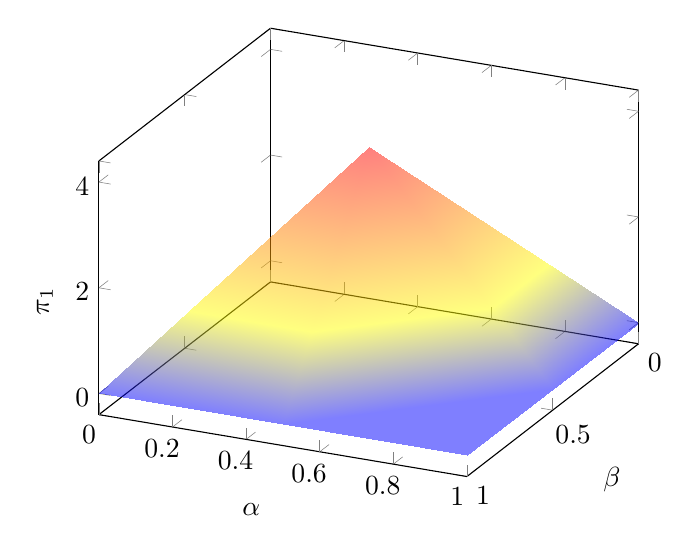
\begin{tikzpicture}
	\begin{axis}[
	xlabel={$\alpha$}, ylabel={$\beta$}, zlabel={$\pi_1$},
	ymajorgrids=false,
	y dir=reverse,
	]
	
	% Best response correspondence of player 1
	\addplot3[surf, shader=interp, mesh/cols=3,opacity=0.5]
	coordinates {(0,0,0) (0.5,0,0) (1,0,0)
				(0,0.5,0) (0.5,0.5,4) (1,0.5,0)
				(0,1,0) (0.5,1,0) (1,1,0)
			};

	\end{axis}
	\end{tikzpicture}
\end{figure}

From the chart, it is straightforward that the best response of player 1 is to set $\alpha = \beta = \frac{1}{2}$. Therefore, the outcome of the game is $y = (2, 2); z = (2, 2)$ with $\pi_1 = 4$ and $\pi_2 = 2$. However, I can't give an explicit expression for SGPE in case where the set of pure strategies is infinite.

\subsubsection*{4.3}

\end{document}
